\documentclass[dvipdfmx]{jsarticle}
\usepackage{tikz}
\usetikzlibrary{intersections,calc,arrows.meta}

\usepackage{amsmath,amsfonts}
\usepackage{bm}

\begin{document}


% \begin{tikzpicture}
%   \draw [dotted,thin] (-2,-2) grid (2,2);
%   \draw [->,thick] (-2.2,0) -- (2.2,0) node [right]{x};
%   \draw [->,thick] (0,-2.2) -- (0,2.2) node [above]{y};
%   \node [below left] (0,0){O};
%   \draw [domain=0:360,smooth] plot (\x:{1-sin(\x)});
%   \end{tikzpicture}


% \begin{tikzpicture}
%   \draw [dotted,thin] (-2,0) grid (2,4);
%   \draw [->,thick] (-2.2,0) -- (2.2,0) node [right]{x};
%   \draw [->,thick] (0,-0.2) -- (0,4.2) node [above]{y};
%   \node [below left] (0,0){O};
%   \draw [domain=-2:2,smooth] plot (\x,{exp(ln(2)*\x)});
%   \end{tikzpicture}

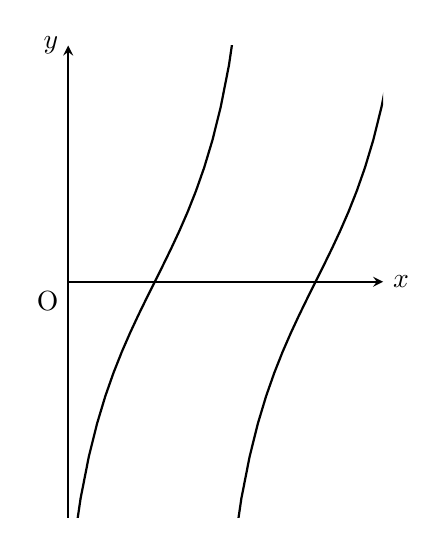
\begin{tikzpicture}
  \draw[->,>=stealth,semithick] (0,0)--(4,0) node[right]{$x$}; %x軸
  \draw[->,>=stealth,semithick] (0,-3)--(0,3) node[left]{$y$}; %y軸
  \draw (0,0) node[below left]{O}; %原点
  \begin{scope}\clip (0,-3) rectangle (4,3);
    \draw[shift={(0.35*pi,0)},thick,domain=-0.4*pi:0.4*pi] plot(\x,{2*tan(\x r)});
    \draw[shift={(pi,0)},thick,domain=-0.4*pi:0.4*pi] plot(\x,{2*tan(\x r)});
  \end{scope}
\end{tikzpicture}

\end{document}